\chapter[Guidelines d'Annotations]{Rendus Techniques : guidelines d'annotations}

Loin d'être destiné à être utilisé tel quel par des annotateurs, ce guide d'annotation de GenHisDoc a pour principal objectif de consigner la méthodologie employée pour produire les annotations et les corrections du jeu de données. Le stage s'étant déroulé entièrement en anglais, l'ensemble des travaux, des échanges et de la documentation technique a été produit dans cette langue. C'est pourquoi certains supports de rendu et documents présentés ici conservent leur terminologie originale en anglais.

\hrulefill

\section{Introduction}

Welcome to this data labelling guide for historical corpora annotation. This document will provide you with all the information and context necessary for your work as an annotator. This document is available to you throughout your assignment and you should refer to it if you have any questions.

We want to produce annotations to train a model to detect different types of content in historical documents. To train the model, the annotations must be as consistent as possible.

\subsection{Context}

Our goal is to create an automated system for extracting visual elements using machine learning technology. For this, we have high-quality data, annotated and manually corrected by human hands.

We are currently working on a study of the dissemination of texts by studying images. In this project, we need only interested in the visual elements and we will completely disregard text.

The page of a historical document is composed of text, illustrations, ornaments and other elements added after the creation of the object, such as glosses, comments, stamps, drawings, traces of wear.

\subsection{Task Definition}

You are an annotator and your goal is to annotate the visual elements of the page. To do this, you will draw straight rectangles around the elements that have a label. The 5 labelling tags are the following : 

\begin{itemize}
    \item 0: "Illustration"
    \item 1: "Ornament"
    \item 2: "Initial"
    \item 3: "Stamp"
    \item 4: "Table"
\end{itemize}


\hrulefill
\section{General rules}


Here are some general rules of good practice for your work.

\subsection{Hug the border of the object as tightly as possible}

A precise annotation like the one shown in the image~\ref{fig:goodfit} captures the entire visual element and is as close as possible to the boundaries to reduce confusion for the machine learning model.

\begin{figure}
    \centering
    \begin{subfigure}{0.48\textwidth}
        \centering
        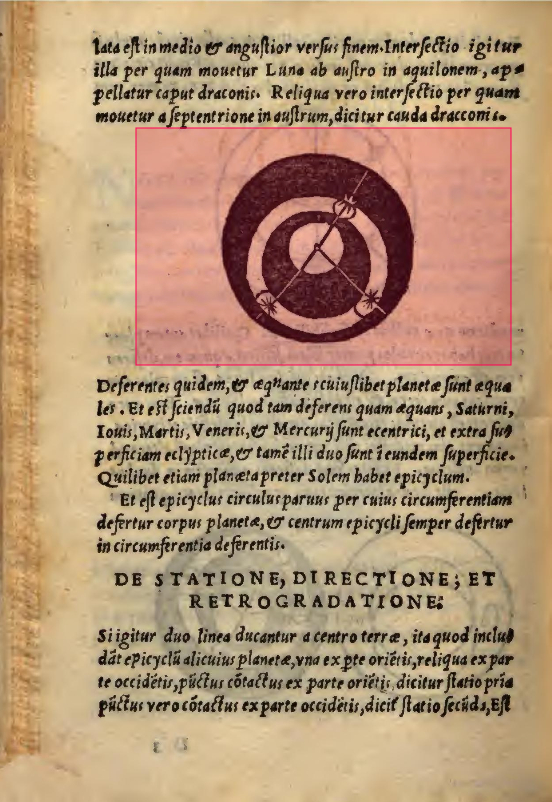
\includegraphics[width=\linewidth, height=7cm, keepaspectratio]{Guidelines/bad_fitting.png}
        \caption{ {\color{red}\faClose} Here, the annotation is too large.}
        \label{fig:badfit}
    \end{subfigure}
    \hfill
    \begin{subfigure}{0.48\textwidth}
        \centering
        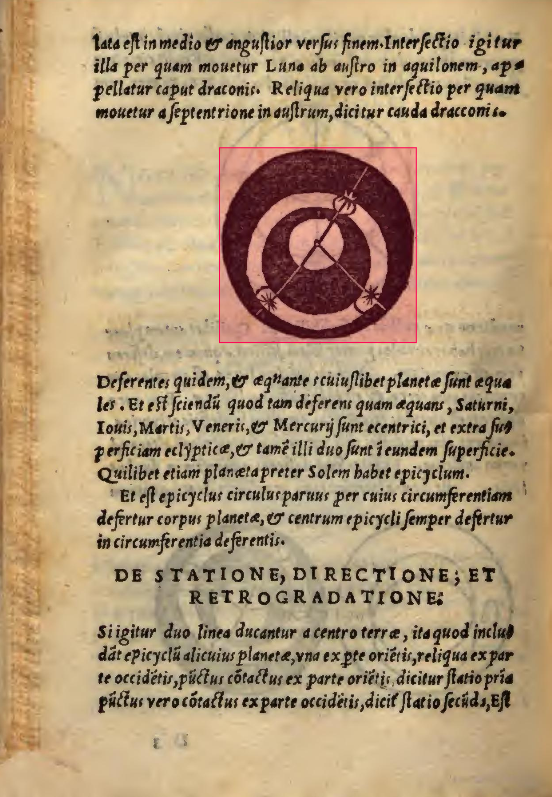
\includegraphics[width=\linewidth, height=7cm, keepaspectratio]{Guidelines/good_fitting.png}
        \caption{ {\color{green}\faCheck} Here is the correct way to annotate an element: the borders are closed to the end of the element without cutting them.}
        \label{fig:goodfit}
    \end{subfigure}
    \caption{Hug the border of the object as tightly as possible.}
\end{figure}

\subsection{Separate the elements that are not visually connected.}

Each distinct visual element must receive its own annotation (bounding box), even if several elements appear to form a coherent whole from the point of view of meaning or composition intended by the author of the document as seen in Figure~\ref{fig:unification} and Figure~\ref{fig:separation}.

Two elements can be "linked" in the author's intention (for example, a human figure and a dog figure accompanying it, or related but non-touching ornamentation) without being visually connected (that is, without sharing a common background, frame, or direct contact). In this case, the annotations are separate.

If several elements share the same background or frame (for example, several symbols or drawings printed on a single continuous graphic strip), they can be grouped into a single annotation, because they are physically or visually unified on the medium as seen in Figure~\ref{fig:example_illustration_frame} and \ref{fig:example_illustration_frame_rule} .

\begin{figure}
    \centering
    \begin{subfigure}{0.48\textwidth}
        \centering
        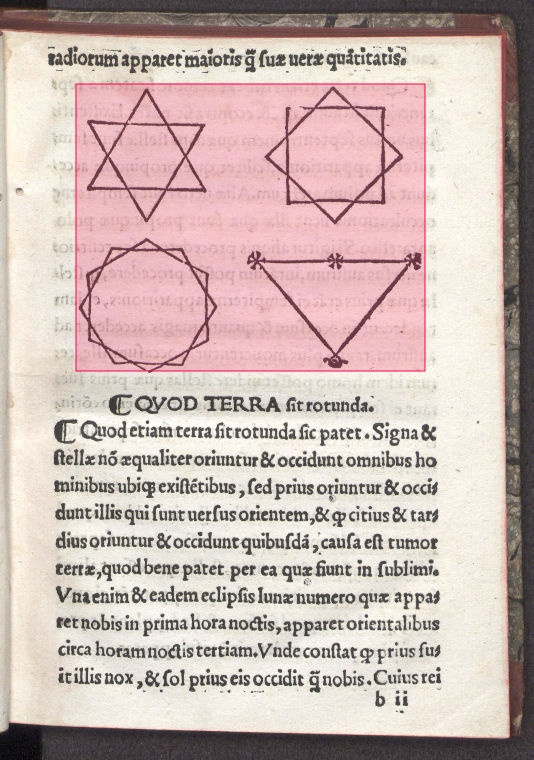
\includegraphics[width=\linewidth, height=7cm, keepaspectratio]{Guidelines/unification.png}
        \caption{{\color{red}\faClose} These elements, although clearly grouped together by the author, should not be annotated in this way.}
        \label{fig:unification}
    \end{subfigure}
    \hfill
    \begin{subfigure}{0.48\textwidth}
        \centering
        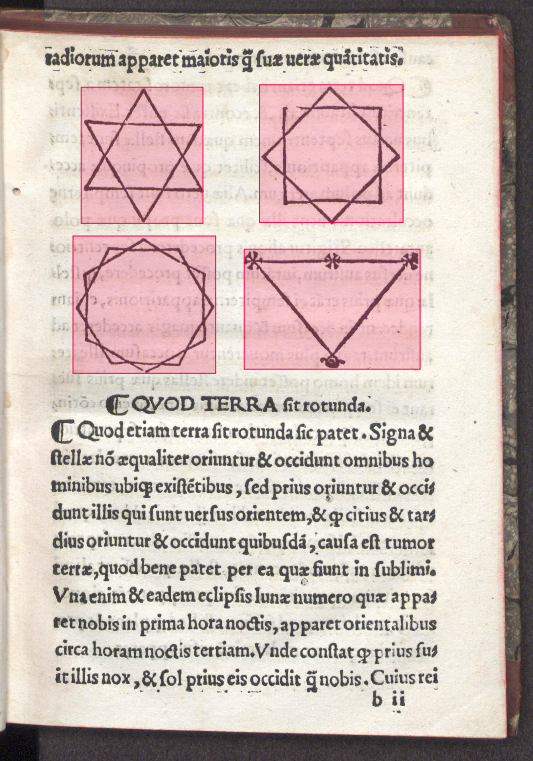
\includegraphics[width=\linewidth, height=7cm, keepaspectratio]{Guidelines/separation.png}
        \caption{{\color{green}\faCheck} Here's how we want to annotate several elements.}
        \label{fig:separation}
    \end{subfigure}
    \caption{Separate element that are not visualy linked}
\end{figure}

\subsection{Avoid item overlap} 

\textbf{This is not a strict rule}. In many documents, elements overlap and are interconnected, as illustrated in Figure \ref{fig:good_overlap}. The section on class definitions and examples will show you the cases where overlapping annotations are necessary and those where they can be avoided.

\begin{figure}
    \centering
    \begin{subfigure}{0.48\textwidth}
        \centering
        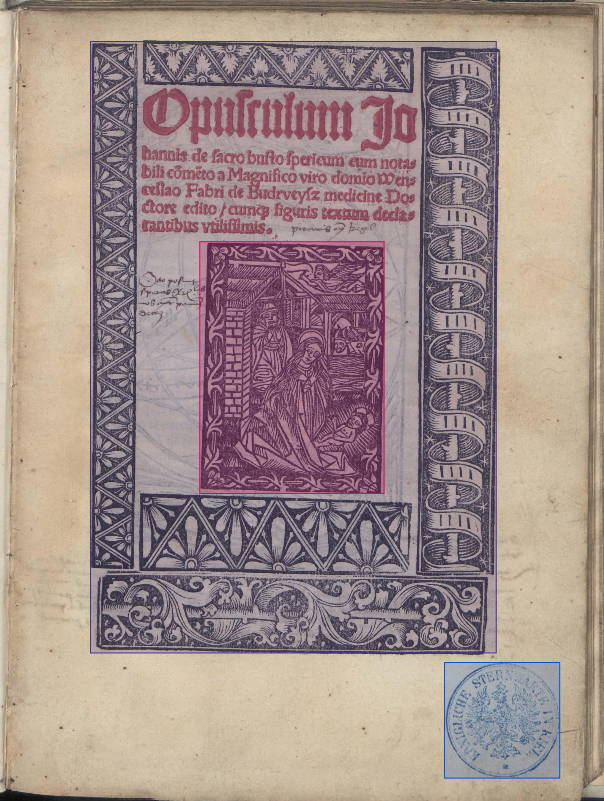
\includegraphics[width=\linewidth, height=7cm, keepaspectratio]{Guidelines/overlap.png}
        \caption{{\color{red}\faClose} The annotation of the ornament overlap against to much elements}
        \label{fig:bad_overlap}
    \end{subfigure}
    \hfill
    \begin{subfigure}{0.48\textwidth}
        \centering
        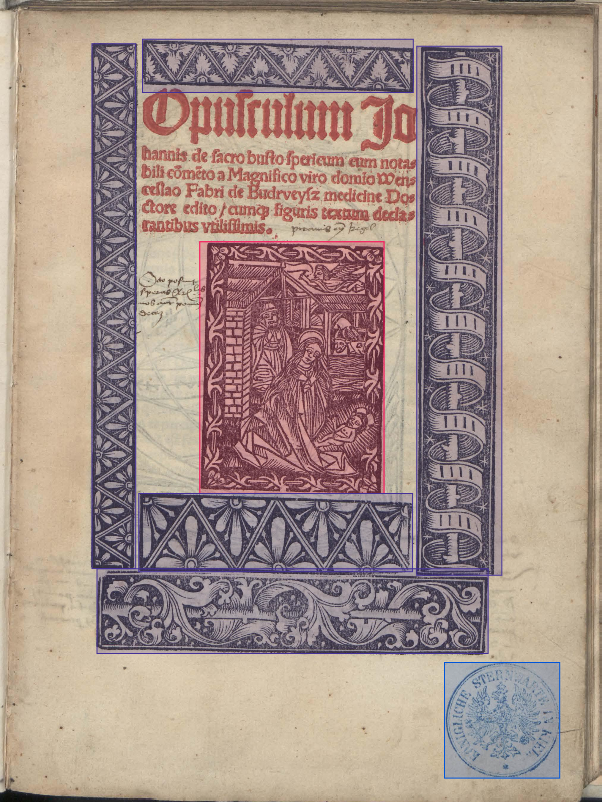
\includegraphics[width=\linewidth, height=7cm, keepaspectratio]{Guidelines/correct_overlap.png}
        \caption{{\color{green}\faCheck} We decided to cut out the decorative elements to avoid overlapping.}
        \label{fig:good_overlap}
    \end{subfigure}
    \caption{Avoid item overlap between classes}
\end{figure}

\subsection{Annotate only the main page}

Do not annotate anything that is not on the main page. As shown in example \ref{fig:main_page}, if the scan was done for two pages, annotate it as shown in \ref{fig:both_page}.

\begin{figure}
    \centering
    \begin{subfigure}{0.48\textwidth}
        \centering
        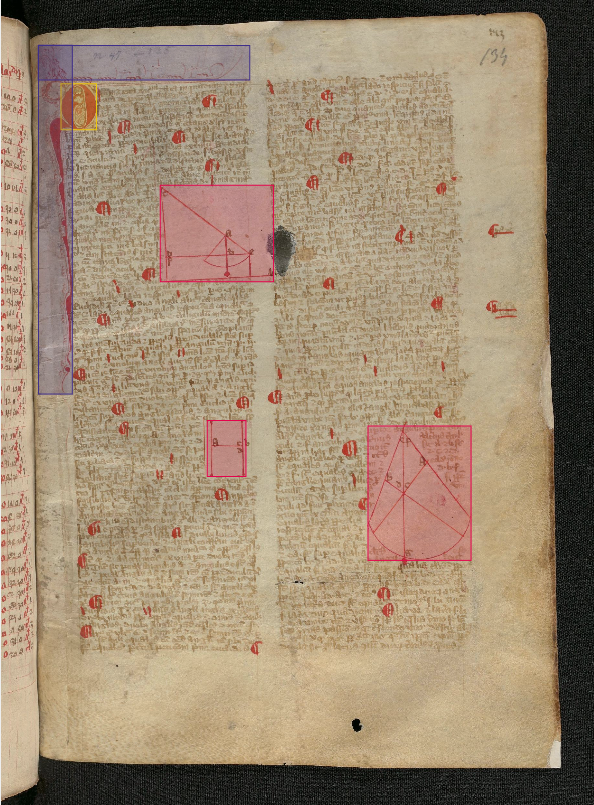
\includegraphics[width=\linewidth, height=7cm, keepaspectratio]{Guidelines/Screenshot_20260702_112821.png}
        \caption{Do not annotate the tables on the little bit of the other page.}
        \label{fig:main_page}
    \end{subfigure}
    \hfill
    \begin{subfigure}{0.48\textwidth}
        \centering
        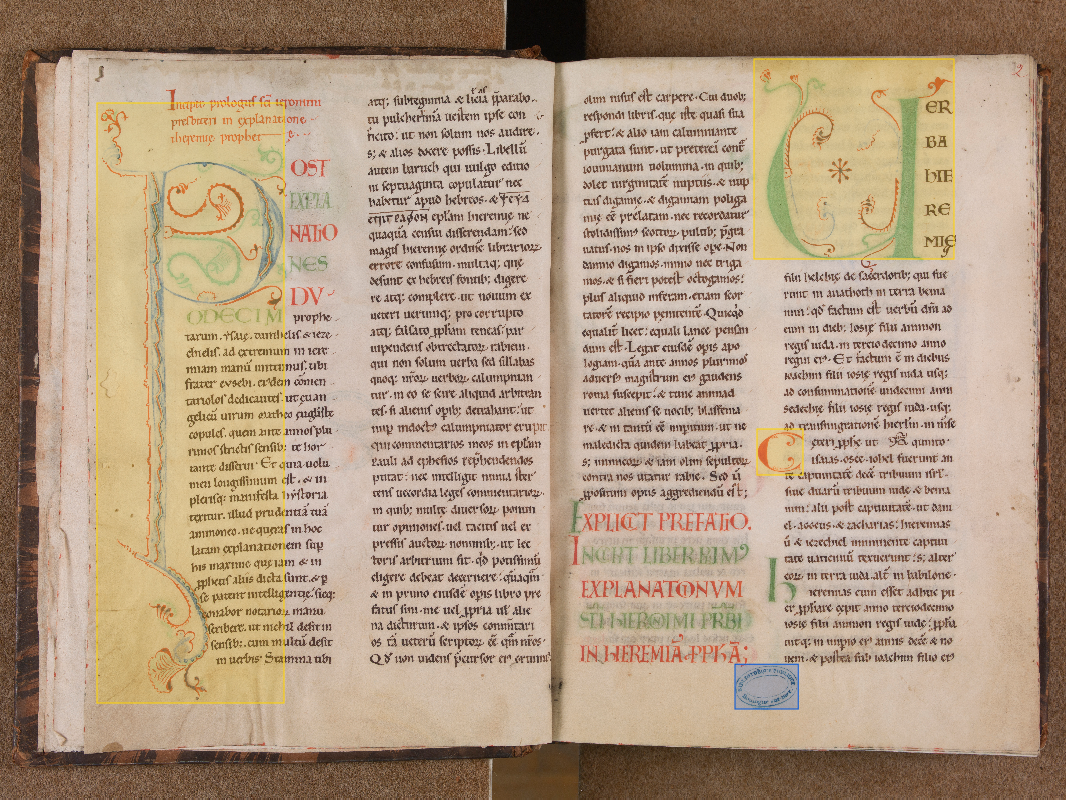
\includegraphics[width=\linewidth, height=7cm, keepaspectratio]{Guidelines/Screenshot_20260702_135302_2.png}
        \caption{If the scan is done for two pages, then you must annotate the elements of both pages.}
        \label{fig:both_page}
    \end{subfigure}
    \caption{Annotate only the main page}
\end{figure}

\subsection{Annotate what is visible, not what you infer}

Label only the content that is actually present and legible in the document, as shown in the image \ref{fig:completion}. Do not extend a bounding box or complete an area based on what you assume to be there (for example, a torn page, an erased stamp, text hidden by a fold).

\begin{figure}
    \centering
    \begin{subfigure}{0.48\textwidth}
        \centering
        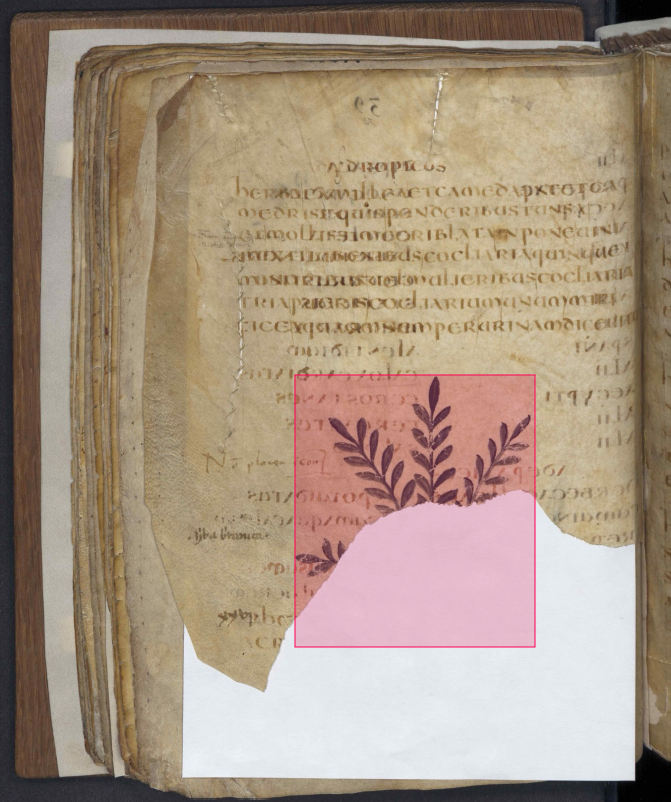
\includegraphics[width=\linewidth, height=7cm, keepaspectratio]{Guidelines/tomuch.png}
        \caption{{\color{red}\faClose} This annotation attempts to complete an element that is no longer visible.}
        \label{fig:completion}
    \end{subfigure}
    \hfill
    \begin{subfigure}{0.48\textwidth}
        \centering
        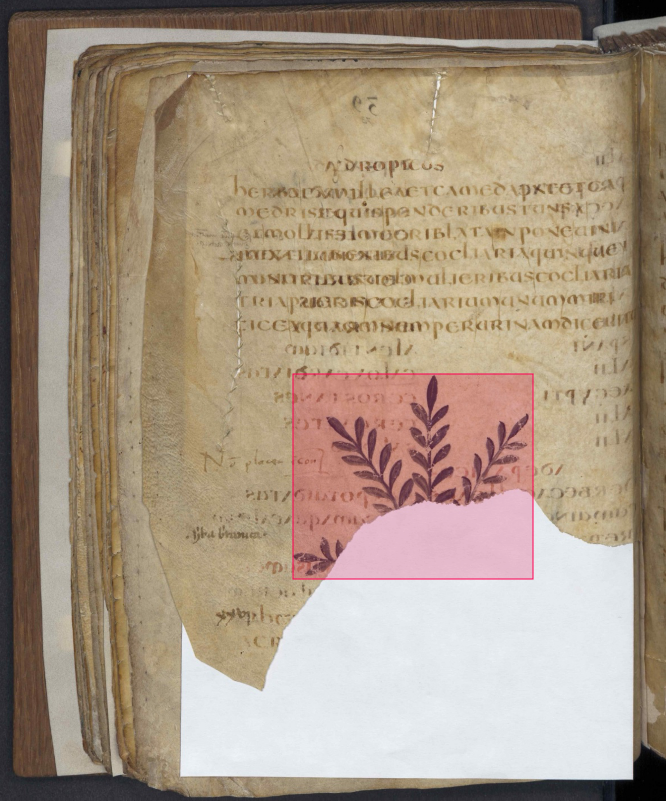
\includegraphics[width=\linewidth, height=7cm, keepaspectratio]{Guidelines/correct_amount.png}
        \caption{{\color{green}\faCheck} This annotation respects the limits of what is visible in the document.}
        \label{fig:fitting}
    \end{subfigure}
    \caption{Annotate what is visible, not what you infer}
\end{figure}

\subsection{Review your work before submitting.}

The annotation task can be arduous and tedious; it is advisable to check the quality of the annotations before moving on to the next image and to take regular breaks to stay alert and focused.

\hrulefill
\section{Class definition}

\begin{comment}

\begin{figure}
    \centering
    \begin{subfigure}{0.48\textwidth}
        \centering
        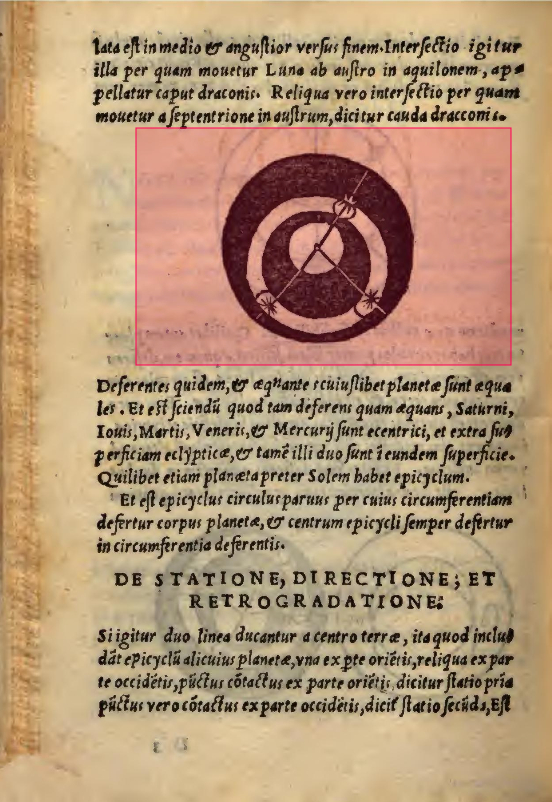
\includegraphics[width=\linewidth, height=7cm, keepaspectratio]{Guidelines/bad_fitting.png}
        \caption{ {\color{red}\faClose} The annotation is too large here.}
        \label{fig:badfit}
    \end{subfigure}
    \hfill
    \begin{subfigure}{0.48\textwidth}
        \centering
        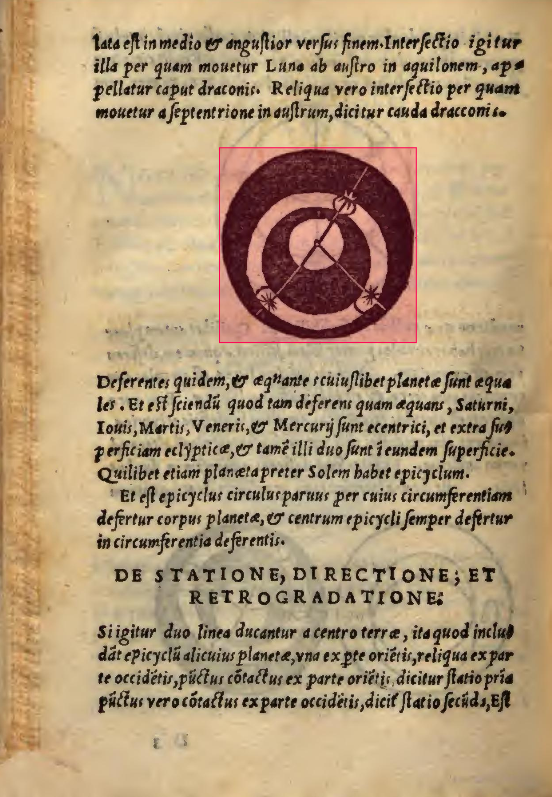
\includegraphics[width=\linewidth, height=7cm, keepaspectratio]{Guidelines/good_fitting.png}
        \caption{ {\color{green}\faCheck} This is the correct way of annotating an element, the borders are close to the end of the element without biting them.}
        \label{fig:goodfit}
    \end{subfigure}

\end{figure}

\end{comment}

You will be annotating the corpus of documents with 5 classes to describe elements inside historical documents:

\subsection{Illustration}

\subsubsection{Description}

The class "illustration" should be understood as a generic class encompassing all graphic elements. An illustration can be functional or artistic; its function is then to inform, illustrate, or entertain the reader.

Examples of illustrations within an image include paintings, photographs, drawings, mathematical graphs, charts, diagrams, symbols, and maps. What distinguishes an illustration from an ornament is its own semantics: it has a meaning that is interpreted in relation to the text, unlike an ornament which is purely decorative.

\begin{figure}
  \centering
  \begin{subfigure}{0.48\textwidth}
    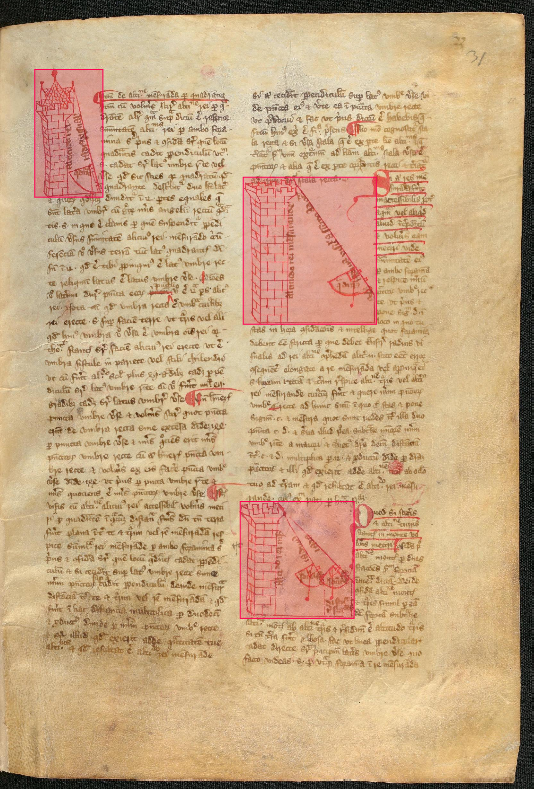
\includegraphics[width=\linewidth, height=7cm, keepaspectratio]{Guidelines/illustraiton_4.png}
    \caption{A geometry manuscript that illustrates angle calculations.}
  \end{subfigure}
  \hfill
  \begin{subfigure}{0.48\textwidth}
    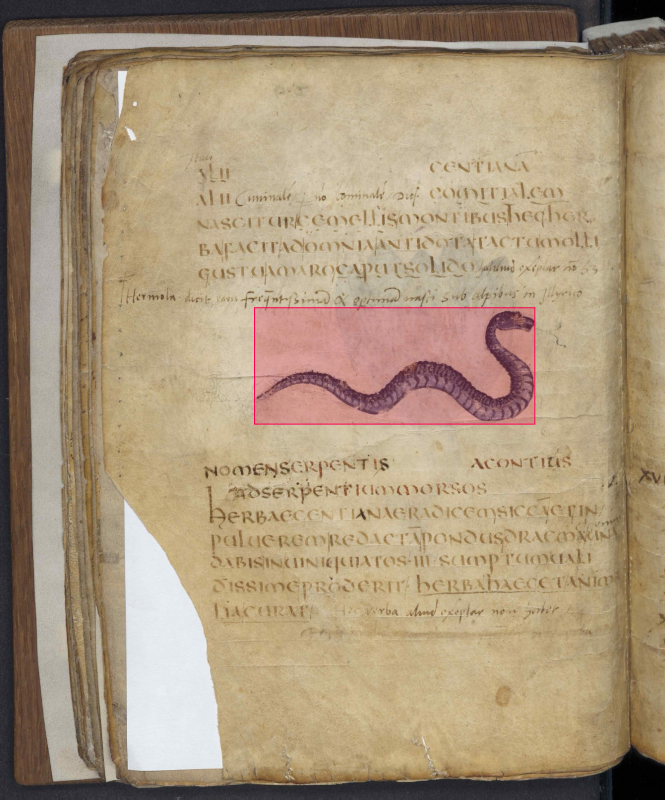
\includegraphics[width=\linewidth, height=7cm, keepaspectratio]{Guidelines/illustration_2.png}
    \caption{A handwritten bestiary with an illustration of a snake.}
  \end{subfigure}
  \hfill
  \begin{subfigure}{0.48\textwidth}
    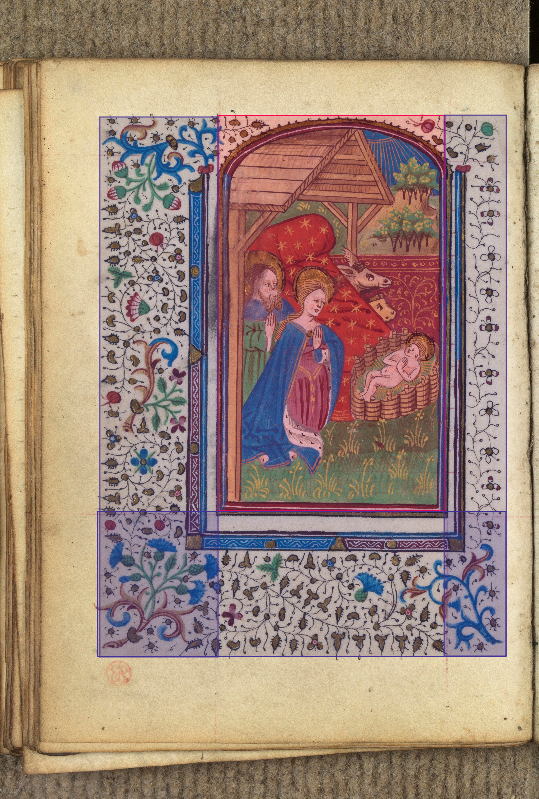
\includegraphics[width=\linewidth, height=7cm, keepaspectratio]{Guidelines/illustration_3.png}
    \caption{a handwritten book of hours with an illustration amidst floral ornamentation.}
    \label{fig:manuscript_bookofhours}
  \end{subfigure}
  \hfill
  \begin{subfigure}{0.48\textwidth}
    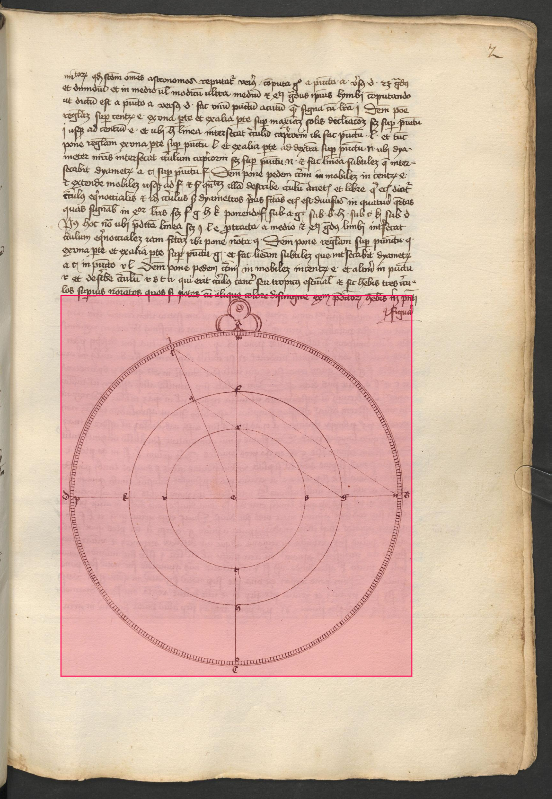
\includegraphics[width=\linewidth, height=7cm, keepaspectratio]{Guidelines/ilustration_5.png}
    \caption{An astronomy manuscript with a mathematical diagrams.}
  \end{subfigure}
  \caption{Illustrations examples}
\end{figure}

\subsubsection{Rules}

The annotations of Illustrations can affected by the layout of the page, they can be grouped and it is hard to understand which ones need to be annotated alone and which ones need to be annotated together.

\begin{itemize}
  \item \textbf{Is there a frame around multiples illustrations ?} : Illustrations in a frame belong together and need to be annotated acordingly. The bounding boxes need to be drawn around the limits of the frame. As shown in this image~\ref{fig:separation}, and shown here~\ref{fig:example_illustration_frame} a grouped illustration without a frame should be separated in multiple annotations. 

  \item \textbf{Is there a common background ?} : If Illustrations share a visual element between them, they need to be annotated together.

  \item \textbf{Do the Illustrations touch ?}: If Illustration touch each other, they need to be annotated together.
\end{itemize}

\begin{figure}
  \centering
  \begin{subfigure}{0.48\textwidth}
    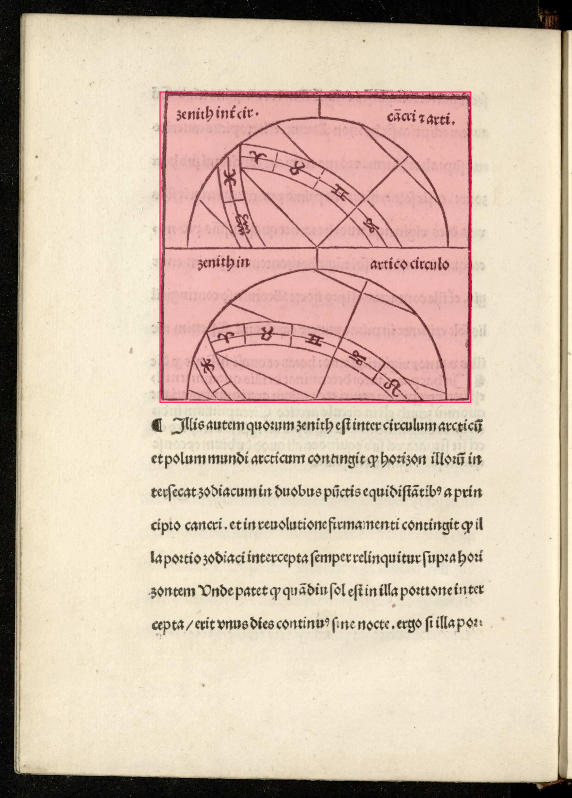
\includegraphics[width=\linewidth, height=7cm, keepaspectratio]{Guidelines/sepsepsep.png}
    \caption{Two illustrations annotated together because they touch and share the same frame.}
    \label{fig:example_illustration_frame}
  \end{subfigure}
  \hfill
  \begin{subfigure}{0.48\textwidth}
    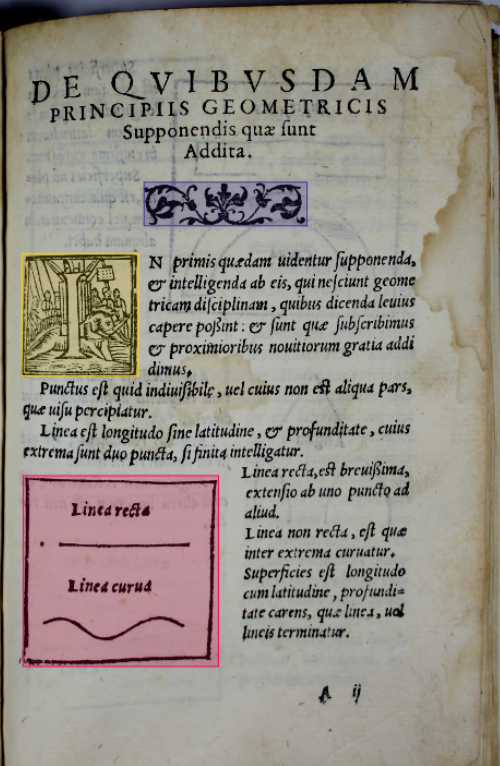
\includegraphics[width=\linewidth, height=7cm, keepaspectratio]{Guidelines/illustration_frame_rule.png}
    \caption{Two illustrations (red) that do not touch but are annotated together because they share a frame.}
    \label{fig:example_illustration_frame_rule}
  \end{subfigure}
  \caption{Edgcases for illustrations}
\end{figure}

\subsubsection{Edgecases}

\begin{itemize}
  \item \textbf{Printer's mark} : A printer's mark is a symbol that was used as a trademark by early printers starting in the 15th century. Printers' marks are often placed on the title page, just below the title and the author's name. The printer's mark should be annotated as an illustration ; see Figure ~\ref{fig:printermark}

  \item \textbf{Illustration and ornamentation} will often be combined into complex visual element. If a visual element is composed by an illustration and an ornamentation, the annotator shoud separate this elements as shown ; see Figures~\ref{fig:manuscript_bookofhours}, \ref{fig:illustration_ornamented_frame} and~\ref{fig:illustration_ornamentation_initial}. 
\end{itemize}


\begin{figure}
  \centering 
  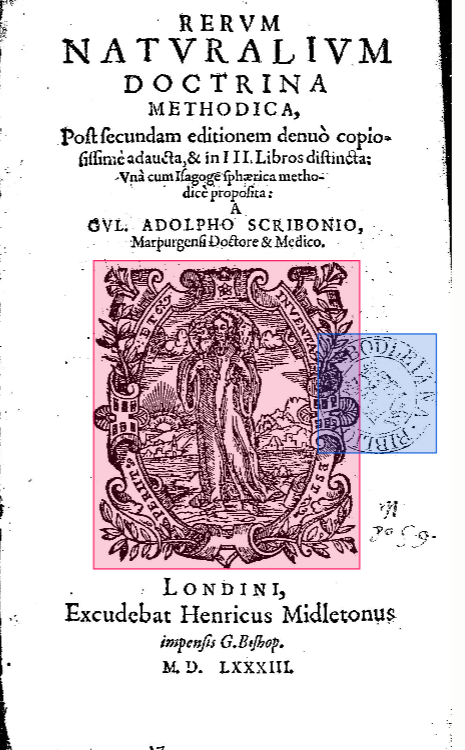
\includegraphics[width=\linewidth, height=7cm, keepaspectratio]{Guidelines/printer_mark.png}
  \caption{A printer's mark on a title page}
  \label{fig:printermark}

\end{figure}



\begin{figure}
  \centering
  \begin{subfigure}{0.48\textwidth}
    \centering
    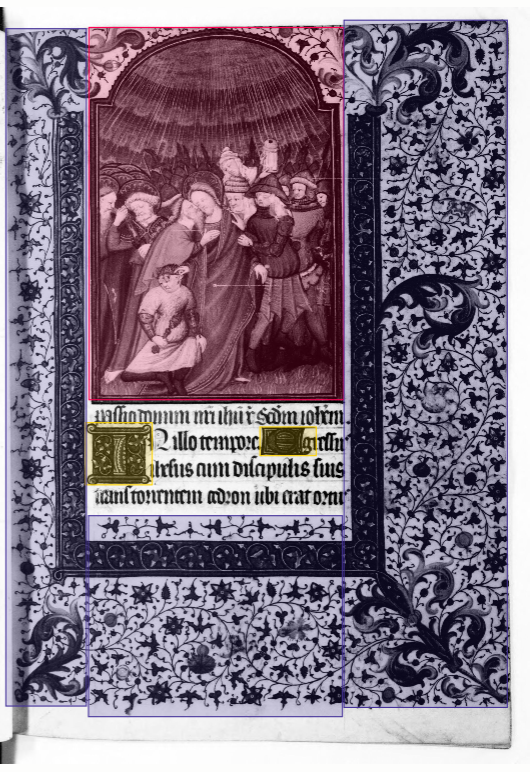
\includegraphics[width=\linewidth, height=7cm, keepaspectratio]{Guidelines/illustration_initial_ornamentation.png}
    \caption{A manuscript that show how to annotate illustration and ornamentation}
    \label{fig:illustration_ornamentation_initial}
  \end{subfigure}
  \hfill
  \begin{subfigure}{0.48\textwidth}
    \centering
    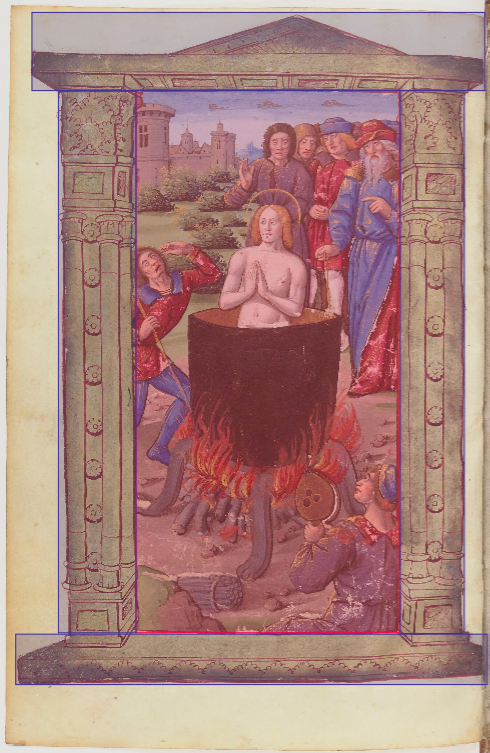
\includegraphics[width=\linewidth, height=7cm, keepaspectratio]{Guidelines/ornamentation_illustration.png}
    \caption{An illustration with an ornamented frame around.}
    \label{fig:illustration_ornamented_frame}
  \end{subfigure}
  \caption{Illustrations and ornaments relationships}
\end{figure}

\subsection{Ornament}\label{section:ornament}
\subsubsection{Description}

An ornament is a graphic element that decorates or embellishes a document without adding informational value.

An ornament is most often an abstract form of illustration, composed of classical patterns (plant ornaments, abstract headpieces, "cul-de-lampe") or repetitive motifs with no meaning other than their intrinsic value as ornaments.

\subsubsection{Rules \& edgecases}

Annotating ornaments is inherently complex, because they frequently interact with and wrap around other elements on the page. Therefore, most ornaments cannot be annotated with a single bounding box. Instead, when an ornament wraps around a visual element (an illustration, a table, a block of text, etc.), it must be \textbf{split into several separate boxes} that follow the contour of the underlying element, rather than being enclosed in one large box that also captures unrelated content.

The following rules apply:

\begin{itemize}
  \item \textbf{The typographic elements for page organization.} (e.g.\ (strokes, bold lines, a simple line or a separator with no complex interaction with the page content) should \textbf{not} be annotated at all.

  \item \textbf{Text inside an ornament} is irrelevant to the annotation: In some manuscripts, there is sometimes text within an ornamental design. Since we are not taking the text into account, these elements must be ornamented normally. Whether or not text appears within the ornamented area does not change how the ornament itself is annotated ; see Figure~\ref{fig:ornament_text}.

  \item \textbf{Ornaments wrapping around another element} must be cut into multiple pieces that follow the shape of that element, instead of a single bounding box ; see Figure~\ref{fig:ornament_1}.

  \item \textbf{Linked/split pieces} resulting from such a cut must be marked with an overlap so that they can later be reconstructed into a single logical ornament ; see Figure~\ref{fig:ornament_overlap}.

  \item \textbf{Ornaments used as separators}, for instance to delimit illustrations or tables from one another, should be annotated as ornaments in their own right ; see Figure~\ref{fig:ornament_tables}.
\end{itemize}

\begin{figure}
  \centering
  \begin{subfigure}{0.48\textwidth}
    \centering
    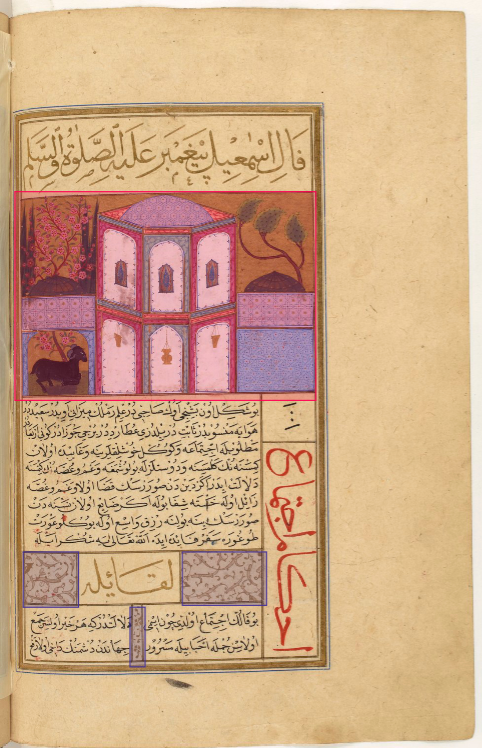
\includegraphics[width=\linewidth, height=7cm, keepaspectratio]{Guidelines/ornament.png}
    \caption{example of ornaments annotations}
    \label{fig:ornament_1}
  \end{subfigure}
  \hfill
    \begin{subfigure}{0.48\textwidth}
    \centering
    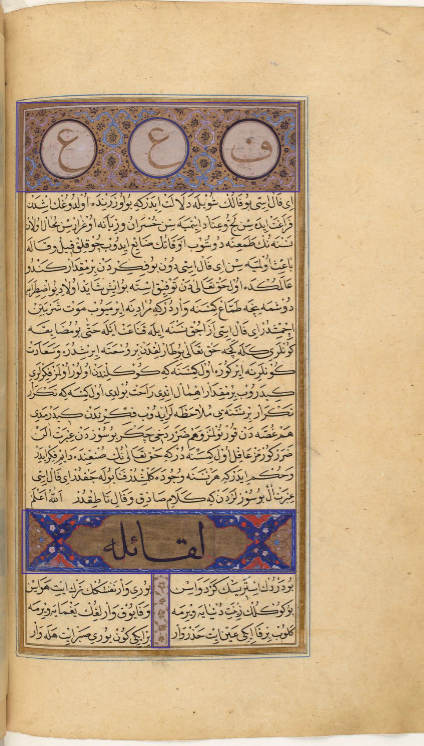
\includegraphics[width=\linewidth, height=7cm, keepaspectratio]{Guidelines/ornament_2.png}
    \caption{We do not care if there is text inside of the ornamentation.}
    \label{fig:ornament_text}
  \end{subfigure}
  \hfill
  \begin{subfigure}{0.48\textwidth}
    \centering
    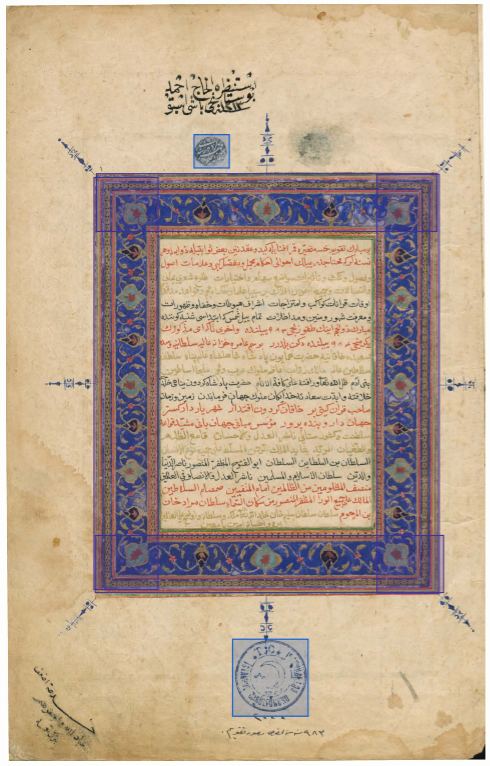
\includegraphics[width=\linewidth, height=7cm, keepaspectratio]{Guidelines/ornament_3.png}
    \caption{When cutting out ornamentation, pieces that are linked together should be marked with overlays so that they can be reconstructed later.}
    \label{fig:ornament_overlap}
  \end{subfigure}
  \hfill
  \begin{subfigure}{0.48\textwidth}
    \centering
    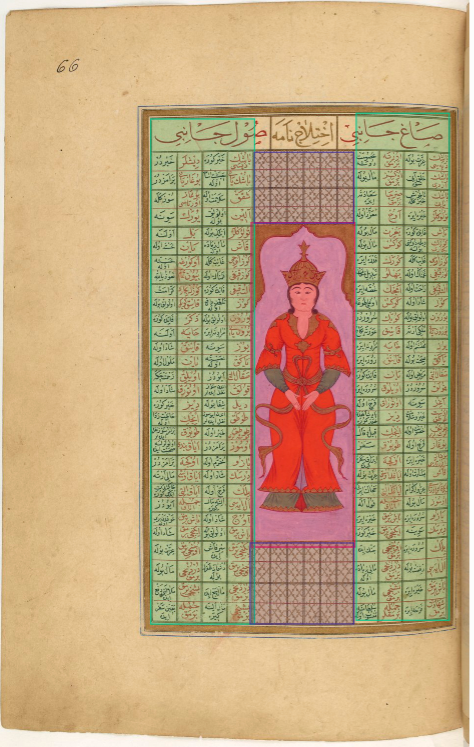
\includegraphics[width=\linewidth, height=7cm, keepaspectratio]{Guidelines/ornament_4.png}
    \caption{Ornamention can be used to separate element like illustrations or tables.}
    \label{fig:ornament_tables}
  \end{subfigure}
  \hfill  
  \begin{subfigure}{0.48\textwidth}
    \centering
    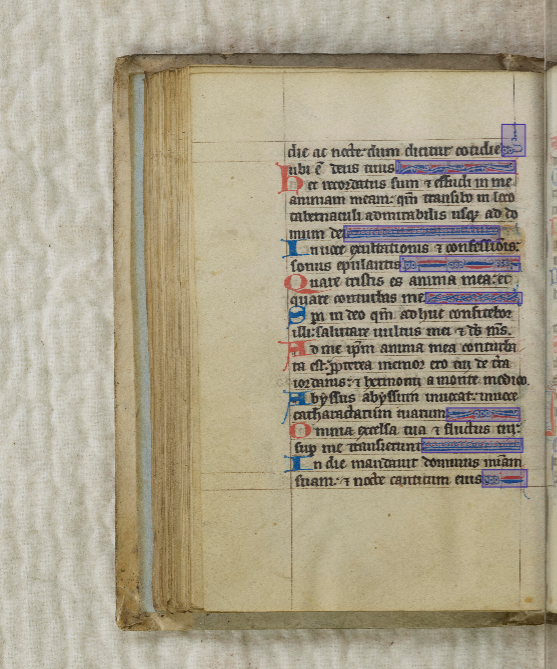
\includegraphics[width=\linewidth, height=7cm, keepaspectratio]{Guidelines/ornament_end_of_line.png}
    \caption{In manuscript, the end of the line can be ornemented}
    \label{fig:ornament_end_of_line}
  \end{subfigure}
  \hfill  
  
  \caption{ornaments examples}
\end{figure}


\subsection{Initial}
\subsubsection{Description}

In a written or manuscript work, an initial is a letter at the beginning of a word, a chapter, or a paragraph that is larger than the rest of the text. An initial is often several lines in height, and, in older books or manuscripts, may take the form of an historiated initial.

\begin{figure}
  \centering
  \begin{subfigure}{0.48\textwidth}
    \centering
    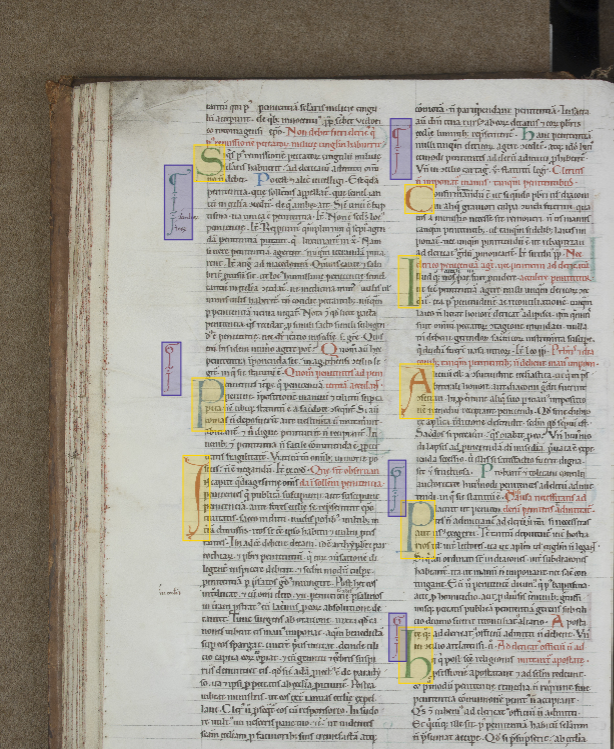
\includegraphics[width=\linewidth, height=7cm, keepaspectratio]{Guidelines/initial.png}
    \caption{example of initials annotations}
    \label{fig:initial_1}
  \end{subfigure}
  \hfill
  \begin{subfigure}{0.48\textwidth}
    \centering
    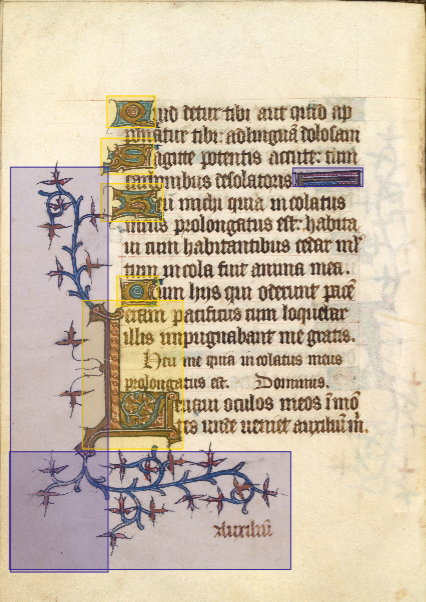
\includegraphics[width=\linewidth, height=7cm, keepaspectratio]{Guidelines/lettrine_ornament.png}
    \caption{Example of the relationship between the initial letter and the ornamentation and how to annotate them.}
    \label{fig:initial_ornament}
  \end{subfigure}
  \hfill
  \begin{subfigure}{0.48\textwidth}
    \centering
    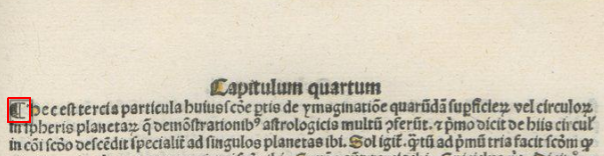
\includegraphics[width=\linewidth, height=7cm, keepaspectratio]{Guidelines/pilcrown_printed.png}
    \caption{Example of a printed pilcrow (¶).}
    \label{fig:printed_pilcrow}
  \end{subfigure}
  \hfill
  \begin{subfigure}{0.48\textwidth}
    \centering
    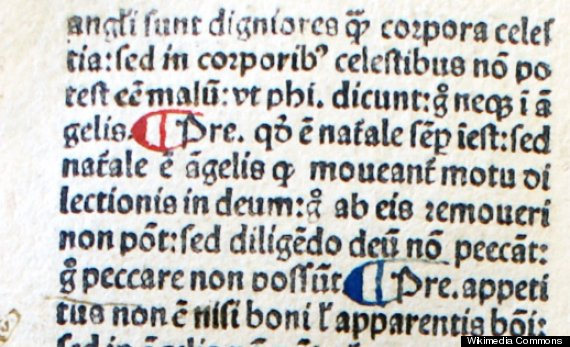
\includegraphics[width=\linewidth, height=7cm, keepaspectratio]{Guidelines/manuscript_pilcrow.jpg}
    \caption{Example of a manuscript pilcrow (¶).}
    \label{fig:manuscript_pilcrow}
  \end{subfigure}
  \hfill
  \caption{Example of initials}
\end{figure}

\subsubsection{Rules}

  An initial is annotated as such only if it is \textbf{visually distinguishable from the body text} typically by a significantly larger size (spanning at least two lines of the surrounding text), a different script, color, or decorative treatment. A letter that is only slightly enlarged compared to the running text should not be annotated as an initial ; see Figure~\ref{fig:both_page}.

\subsubsection{Edgecases}

Initials are letters and therefore can be tricky to annotate due to their textual nature.

\begin{itemize}
  \item \textbf{Initial letter can be used in manuscripts as a basis for marginal ornamentation}. We annotate the initial letter in a "cautious" manner, limiting ourselves to the actual initial letter, and we annotate the rest of the ornamentation using the ornamentation class ; see Figures~\ref{fig:main_page} and \ref{fig:illustration_ornamentation_initial}.

  \item \textbf{Initial capitals can be confused with the paragraph mark (pilcrow ¶)} frequently used in manuscripts. Often written in ink of a different color than the text (red), the pilcrow should not be annotated like an initial capital ; see Figures~\ref{fig:printed_pilcrow}, \ref{fig:manuscript_pilcrow}.
\end{itemize}

\subsection{Stamp}

Stamps are marks that identify the institutions that hold or held the documents (libraries, archives). These markings are not all the same depending on the document and the date they were applied to the work. For bound documents (books, manuscripts, albums), the stamp is on the first page. For a stack of unbound documents, each loose page will be stamped. 

\begin{figure}
  \centering
  \begin{subfigure}{0.48\textwidth}
    \centering
    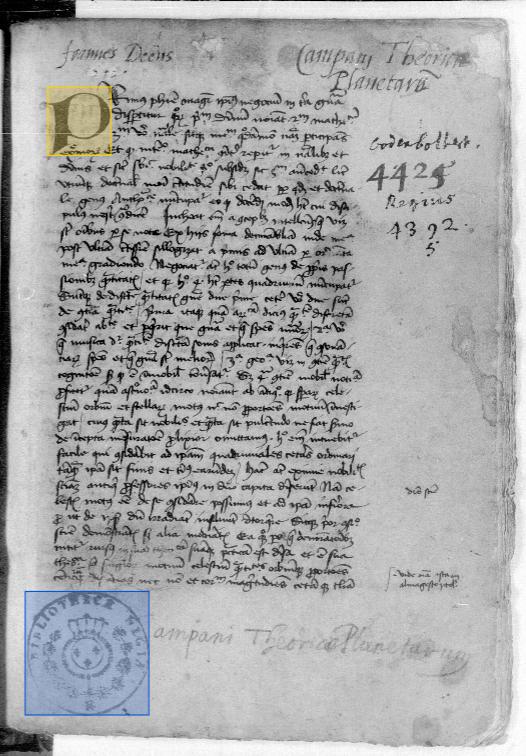
\includegraphics[width=\linewidth, height=7cm, keepaspectratio]{Guidelines/stamp_ex_libris.png}
    \caption{example of a stamp covering his old bookplate.}
    \label{fig:stamp_ex_libris}
  \end{subfigure}
  \hfill
  \begin{subfigure}{0.48\textwidth}
    \centering
    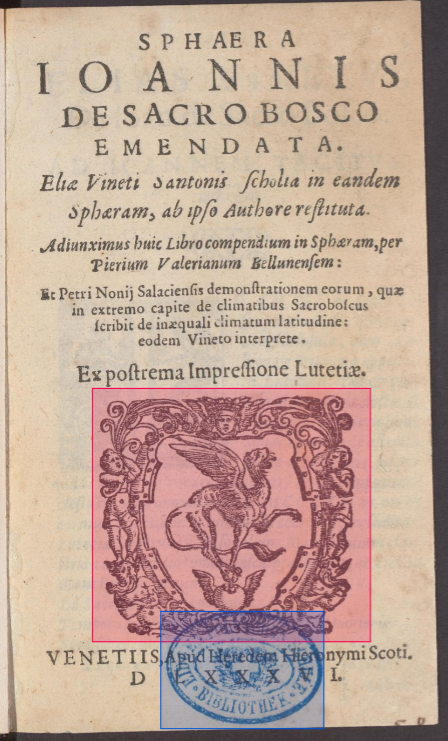
\includegraphics[width=\linewidth, height=7cm, keepaspectratio]{Guidelines/stamps.png}
    \caption{example of a stamp on a title page.}
    \label{fig:stamp_1}
  \end{subfigure}
  \hfill
  \begin{subfigure}{0.48\textwidth}
    \centering
    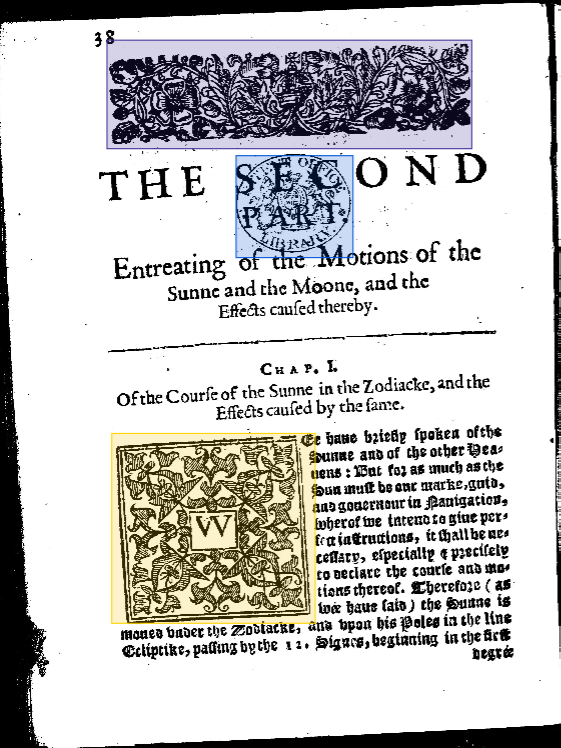
\includegraphics[width=\linewidth, height=7cm, keepaspectratio]{Guidelines/stamps_2}
    \caption{example of a stamp on a first page.}
    \label{fig:stamp_2}
  \end{subfigure}
  \hfill
  \begin{subfigure}{0.48\textwidth}
    \centering
    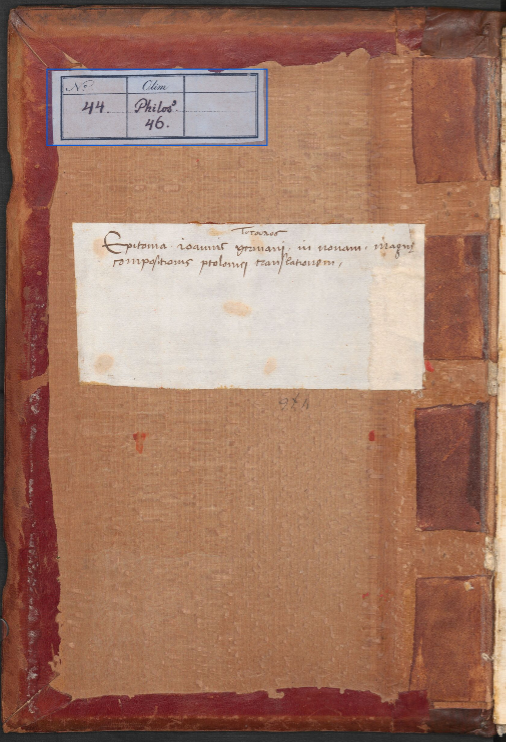
\includegraphics[width=\linewidth, height=7cm, keepaspectratio]{Guidelines/library_stamp.png}
    \caption{example of a library label}
    \label{fig:label}
  \end{subfigure}
  \hfill
  \caption{Example of stamps and library labels}
\end{figure}

\subsubsection{Rules}

\begin{itemize}
  \item \textbf{Annotate all visible stamps}: manuscripts and old books in France have moved between several librairies and therefore often have several stamps which need to be annotated ; see Figure~\ref{fig:stamp_1} and \ref{fig:stamp_2}.

  \item \textbf{Ex-Libris }: Before the widespread use of the stamp, book owners used a handwritten Ex-Libris on the title page; this phrase should not be annotated as a stamp even if it serves the same purpose ; see Figure~\ref{fig:stamp_ex_libris}.

  \item In addition to library stamps, the stamp class is also used to annotate library labels ; see Figure~\ref{fig:label}.
\end{itemize}

\subsection{Table}

A table is an arrangement of information or data, usually in rows and columns, or possibly according to a more complex structure. 

For tables, the header and the footer must included in the annotation if it is present. 

\subsubsection{Rules}

\begin{itemize}
  \item \textbf{The bounding box must include the entire table structure}, including the \textbf{header and footer} rows if present, as well as any surrounding \textbf{border or frame} that is part of the table itself ; see Figure~\ref{fig:tabula_with_title}.

  \item If the table has a \textbf{title or caption} that is graphically separated from the table body (e.g.\ placed above or below it, not enclosed by the table's border), it should \textbf{not} be included in the annotation ; only the tabular structure itself is annotated ; see Figure~\ref{fig:tabula_initial}.

  \item Tables with \textbf{non-rectangular or non-linear structure} (e.g.\ circular tables, radial diagrams used to present structured information such as genealogies or calendars) must still be annotated as tables, using a bounding box that encloses the full extent of the structure.

  \item If a page contains \textbf{several distinct tables} (not visually merged and separated by clear spacing, text, or ornamentation), each table should be annotated separately, even if they share the same overall topic or are placed side by side : see Figure~\ref{fig:tabula_ornement}.

  \item If a table is \textbf{split across a page break or a column break} but is visually one continuous table (repeated headers, continued numbering, etc.), each visible portion is annotated as a separate instance, since annotation is done per visible bounding region.
\end{itemize}

\subsubsection{Edgecases}

\begin{itemize}
  \item \textbf{Tables can be difficult to distinguish from simple lists or aligned text} (e.g.\ an index, a table of contents, or enumerated items with aligned page numbers). A table should only be annotated when there is a clear multi-column/multi-row structure with at least two dimensions of organization ; a single column of aligned entries should not be annotated as a table.

  \item \textbf{Tables can be enclosed or decorated with ornamentation} (borders, frames, or historiated elements). In this case, only the tabular content and its structural border are annotated as a table ; any additional decorative ornamentation surrounding it should be annotated separately using the ornamentation class, following the same logic as for illustrations (see Section~\ref{section:ornament}).

  \item \textbf{Tables with a circular or radial representation} of information (frequent in historical documents, e.g.\ astronomical or genealogical diagrams) should be annotated as tables rather than as illustrations, even though they may visually resemble diagrams or figures.

  \item \textbf{Indexes} and content tables should not be annotated.
\end{itemize}

\begin{figure}
  \centering
  \begin{subfigure}{0.48\textwidth}
    \centering
    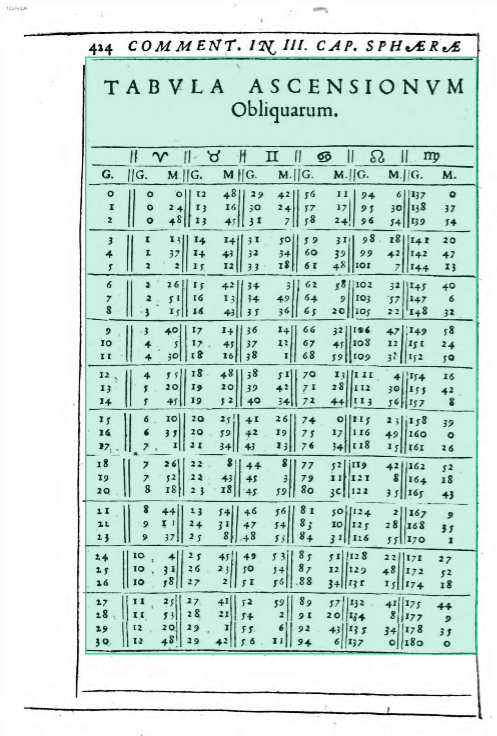
\includegraphics[width=\linewidth, height=7cm, keepaspectratio]{Guidelines/table_1.png}
    \caption{example of an annotated tablewith title}
    \label{fig:tabula_with_title}
  \end{subfigure}
  \hfill
  \begin{subfigure}{0.48\textwidth}
    \centering
    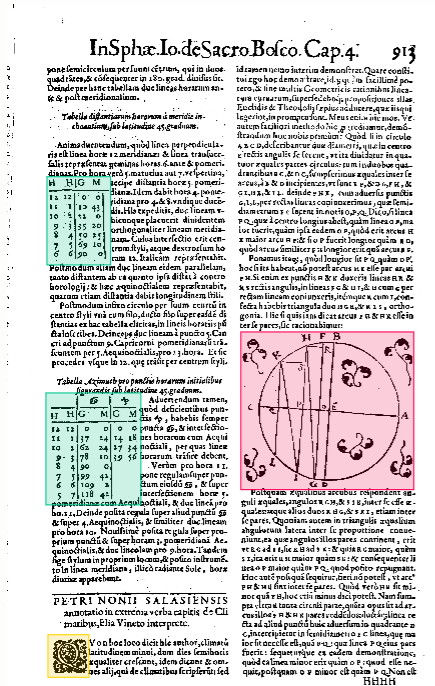
\includegraphics[width=\linewidth, height=7cm, keepaspectratio]{Guidelines/table_2.png}
    \caption{example of tables inserted into the text .}
    \label{fig:tabula_text}
  \end{subfigure}
  \hfill
  \begin{subfigure}{0.48\textwidth}
    \centering
    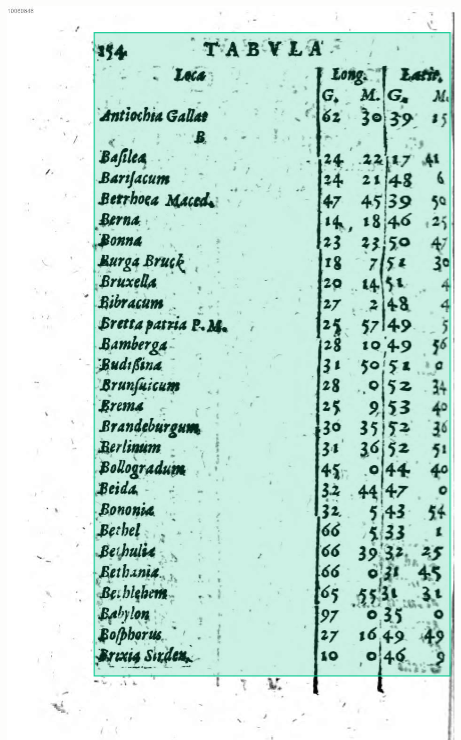
\includegraphics[width=\linewidth, height=7cm, keepaspectratio]{Guidelines/table_3.png}
    \caption{example of a table.}
    \label{fig:tabula_example}
  \end{subfigure}
  \hfill
  \begin{subfigure}{0.48\textwidth}
    \centering
    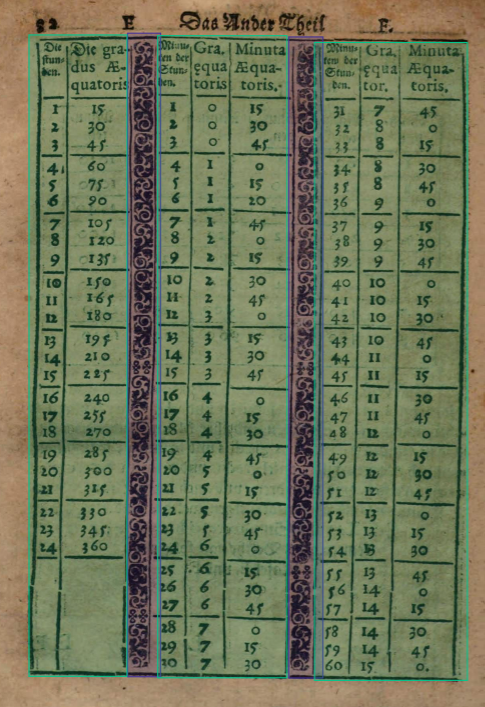
\includegraphics[width=\linewidth, height=7cm, keepaspectratio]{Guidelines/table_6.png}
    \caption{example of tables with ornement.}
    \label{fig:tabula_ornement}
  \end{subfigure}
  \hfill
  \begin{subfigure}{0.48\textwidth}
    \centering
    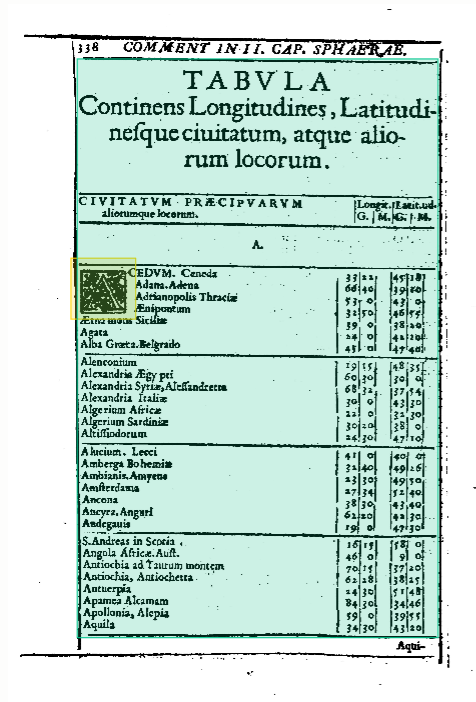
\includegraphics[width=\linewidth, height=7cm, keepaspectratio]{Guidelines/table_7.png}
    \caption{example of a a table with an initial.}
    \label{fig:tabula_initial}
  \end{subfigure}
  \hfill
  \caption{Example of tables}
\end{figure}

